\section{Installation, Integration and Commissioning}
\label{sec:dp-pds-installation}

\subsection{Transport and Handling}

The transportation of the \dwords{pmt} will be on a standard EUR size pallet of dimensions \SI{1.2}{\m} $\times$ \SI{1}{\m}. The largest capacity commercially available box is exemplified in Fig.~\ref{fig:dppd_11_2}. The box can contain \num{36} \dwords{pmt} in three levels of \num{4} $\times$ \num{3} arrays. Individual \dwords{pmt} will be placed in carton boxes with their bases, support structures and short \dword{hv} cables soldered to the bases at the production/assembly sites. \num{36} \dwords{pmt} will then be placed in the transport boxes for shipping to \dword{itf}.

\begin{dunefigure}[An example transportation box envisaged to be used for all transport purposes i.e. from remote sites to the \dword{itf} and from \dword{itf} to \surf.]{fig:dppd_11_2}
{An example transportation box envisaged to be used for all transport purposes i.e. from remote sites to the \dword{itf} and from \dword{itf} to \surf.}
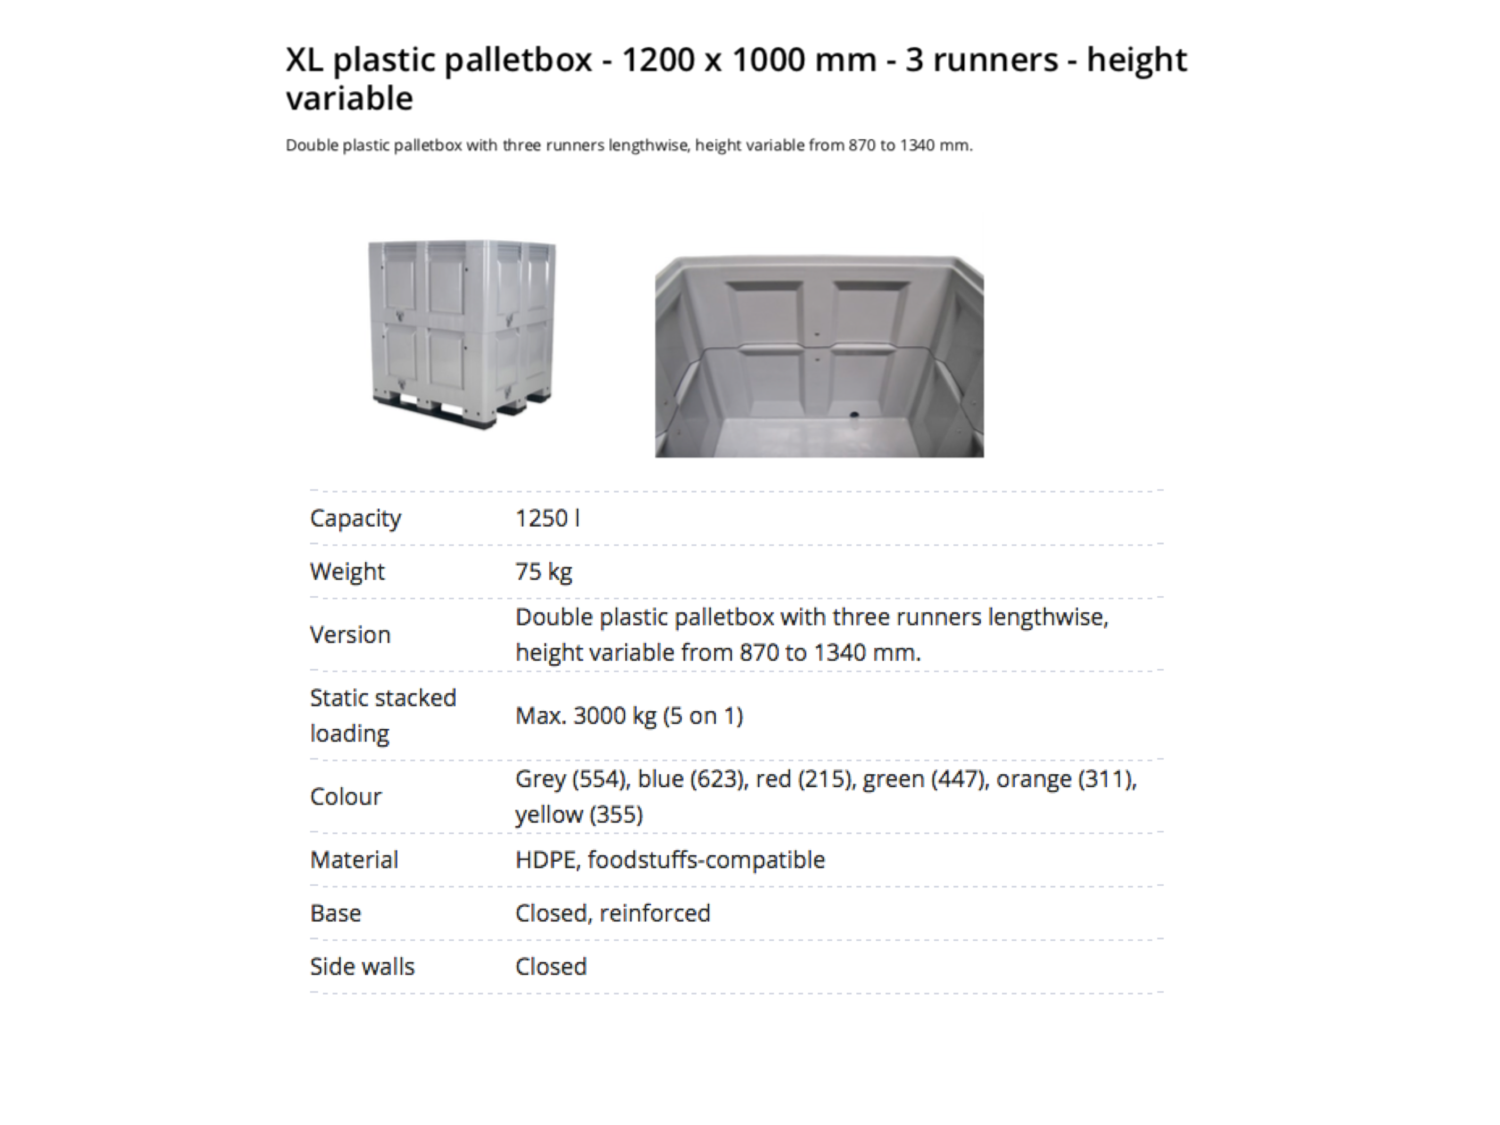
\includegraphics[width=0.5\textwidth]{dppd_11_2}
\end{dunefigure}

Following the \dword{itf} operations, the \dwords{pmt} in arrays of \num{4} $\times$ \num{3} will be placed in a custom structure. The structure will be assembled with metal and plastic parts so that the entire structure together with the \dwords{pmt} can be moved into the clean room underground. Three of these structures will be placed on top of each other inside the boxes with the crane. The individual carton boxes of the \dwords{pmt} will be recycled at the \dword{itf}. The local movement of the transportation boxes in the \dword{itf} area and also within the \dual \dword{pds} work area can be done with compact warehouse-type forklifts. The \dword{pds} work area will also be used as the storage area for the large \dword{pmt} transportation boxes before being sent to \surf. The boxes will be stored in the single-shelf racks to the right and left of the entrance of the work area. The first set of boxes will be placed on the floor and the second set will be on the shelf which is \SI{1.5}{\m} higher off the ground. This area is capable of storing the entire \dual \dword{pds} \dword{pmt} inventory of \dpnumpmtch \dwords{pmt} in \num{20} boxes. The \num{80} spare \dwords{pmt} can be placed in two boxes and the shelves, and the boxes can be stored on the floor in the available space in the work area towards the end of the \dual \dword{pds} \dword{itf} operations.

The large \dword{pds} boxes will be wrapped with plastic foil at the \dword{itf} to be opened in SAS underground. After removal of the plastic wrapping, the transport boxes will be moved to the cleanroom with its entire content. The \dword{pds} boxes can be moved in the underground areas with a pallet jack. The \num{4} $\times$ \num{3} structure will be taken out of the transportation box and moved inside the cleanroom by the crane. The structure will go in the dark box for the functionality tests of the \num{12} \dwords{pmt}. The transportation boxes will be used for storage prior to the installation. The empty boxes will be sent back to \dword{itf}. There will be at most three \dword{pds} boxes in the cleanroom.

The \num{4} $\times$ \num{3} structure will be moved into the cryostat by the crane and will be placed on the cryostat floor at a convenient location with respect to the active installation area. The \dwords{pmt} will then be installed one by one. 

\subsection{Integration and Testing Facility Operations}
\label{subsec:dp-pds-itf}

At the \dword{itf}, \dword{pds} will have a work area with size \SI{10}{\m} $\times$ \SI{8}{\m} and \SI{3.6}{\m} (\SI{12}{\ft}) ceiling including a gantry crane. The work area will be utilized for \dword{tpb} coating of the \dword{pmt} windows, quality control of the \dwords{pmt}, storage and preparation for the transport to \surf. In addition, the installation of individual ground grids on the \dwords{pmt} is under discussion between the \dword{pds} and \dword{hv} consortia. If realized, the mounting of the ground grids on the \dword{pmt} support structures will also be performed at the \dword{itf}.

The layout of the \dword{pds} work area at the \dword{itf} is shown in Fig.~\ref{fig:dppd_11_3}. Two coating stations of \SI{1.5}{\m} $\times$ \SI{1.5}{\m} are envisaged.

\begin{dunefigure}[The layout of the \dword{pds} work area at the \dword{itf}.]{fig:dppd_11_3}
{The layout of the \dword{pds} work area at the \dword{itf}.}
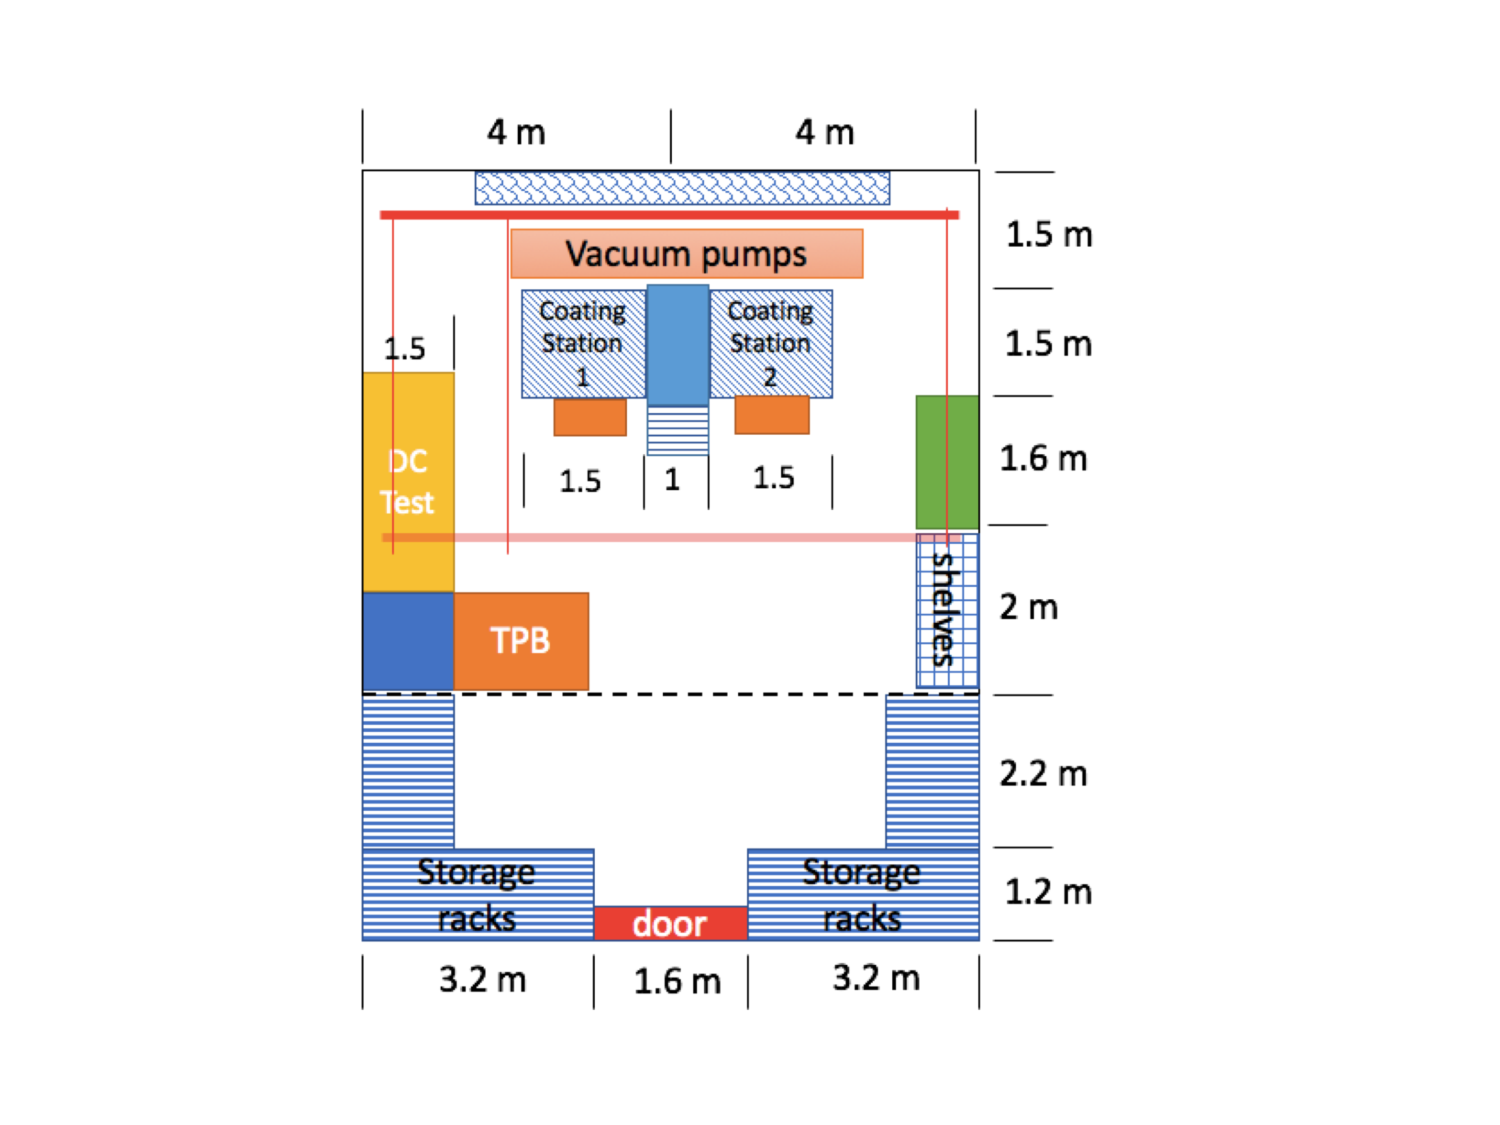
\includegraphics[width=0.4\textwidth]{dppd_11_3}
\end{dunefigure}

Figure ~\ref{fig:dppd_11_4} shows pictures of a \dword{tpb} coating station at the CERN Thin Film Facility. Between the two coating stations, an elevated platform that will be accessed with short stairs will be placed at the \dword{itf} \dword{pds} work area. This platform will be used to conveniently reach the top lid of the evaporator (approximately \SI{1.5}{\m} high from the ground level) and inside the vessel. Cooling water, nitrogen and electricity will be provided from the outlets placed along the \SI{8}{\m} wall (indicated as the area with wavy lines in Fig.~\ref{fig:dppd_11_3}). Vacuum pumps will be placed in the immediate vicinity of the evaporators. Control electronics will also be placed next to the evaporator chambers. 

\begin{dunefigure}[Pictures of a single \dword{tpb} coating station (courtesy of Wil Vollenberg, CERN-TE Department).]{fig:dppd_11_4}
{Pictures of a single \dword{tpb} coating station (courtesy of Wil Vollenberg, CERN-TE Department).}
\includegraphics[width=0.8\textwidth]{dppd_11_4}
\end{dunefigure}

The \dwords{pmt} will be taken out of their individual carton boxes when they arrive at the \dword{itf}. The \dwords{pmt} will be tested for basic functionality in their carton boxes to validate the safe transport from the remote sites and will be kept in these boxes before the coating operations. The \dword{pmt} windows will be cleaned with acetone and isopropanol before the evaporation. This will be performed in the flow device/fume hood shown as a green box along the \SI{10}{\m} wall. The gantry crane (indicated with red bars) will be capable of moving parts between the coating stations and the work desks. It will be used to remove the vessel lid and support it during the installation of the \dword{pmt} for coating.

Following the evaporation procedure, an acrylic protective plate will be installed covering the coated \dword{pmt} windows, and the \dwords{pmt} will be placed in individual dark plastic protective bags. The \dwords{pmt} will go through another round of basic functionality test before being transported to the underground areas. They will then be attached to the \num{4} $\times$ \num{3} structure for transportation to \surf.

At the \dword{itf}, the \dword{pmt} windows will be coated at a rate of \num{4} \dwords{pmt}/day resulting in \num{20} \dwords{pmt}/week and \num{80} \dwords{pmt}/month. Given the installation rate of \num{96} \dwords{pmt}/month, the \dword{itf} operations should start ahead of the start of the installation. The \dword{pds} work area at the \dword{itf} has sufficient storage capacity for the entire \dword{pmt} inventory of the \dword{pds}. 

\subsection{Underground Installation and Integration}
\label{subsec:dp-pds-undergroundinstallation}

The cryostat cable/fiber installation will precede the installation of the field cage. The cables/fibers will be routed from the flanges to the bottom of the cryostat. The total cable/fiber mass (length) is approximately \SI{50}{\kg} (\SI{25}{\m}) per sector with an average mass/length of \SI{2}{\kg/\m}, where one sector comprises \num{36} \dwords{pmt}, see Sec.~\ref{sec:dp-pds-overview_layout}. The free ends of the cables/fibers will be temporarily mounted to the cryostat floor in such a way that they will be easily accessed during installation. The cable/fiber and tray installation will be done on both sides of the cryostat. At this stage, the \dword{hv} cables will be transported in a single box from the \dword{itf} to \surf. At the same time, a separate box containing the \num{120} calibration fiber + fiber bundle assemblies will be transported from the \dword{itf} to \surf. The boxes will be transported to the cryostat roof for hanging the cables/fibers through the feedthroughs for installation in the cable trays.  

Once the plastic wrap is taken off, the \dword{pds} \dword{pmt} box and its entire content can be transported to the clean room. The \dwords{pmt} will undergo functionality tests inside the custom design dark box which can cover the entire structure of \num{4} $\times$ \num{3} \dwords{pmt}. The dark box will have high voltage patch panel and will allow consecutive tests of all \num{12} \dwords{pmt} in one testing session without intervention. The test will be a simple check of healthy \dword{pmt} operations. Once the operation of the \dwords{pmt} is validated, the structure can be moved inside the cryostat.

Inside the cryostat, the \dwords{pmt} will be removed from the structure. The window protections will be kept on the \dwords{pmt}. The \dwords{pmt} will be mounted on the membrane floor, in the areas between the membrane corrugations, through their support structures. The attachment is done via a stainless steel supporting base that could be point-glued to the membrane. The weight of the support and \dword{pmt} exceeds the buoyancy force of the system. Furthermore, these supports also ensure stability against possible lateral forces acting on the \dwords{pmt} due to the liquid flow. Once the fixation is completed, the short \dword{hv} cables will be connected to the cold \dword{hv} cables with SHV barrel connectors. The calibration fibers will be routed and connected to the support structure. Once all the \dwords{pmt} of a given \dword{pds} sector are installed, the cables and fibers will be fixed in their final positions.

The installation will be done at a rate of \num{24} \dwords{pmt}/week. After the installation, the empty \dword{pmt} boxes and the transport structures will be transported back to \dword{itf}. This transportation can be synchronized with the other installation.

Below table summarizes the quantities related to the \dual \dword{pds} installation.

\begin{dunetable}
[Quantities related to the \dual \dword{pds} installation.]
{lc p{0.8\textwidth}}
{tab:dppd_t_11_1}
{Quantities related to the \dual \dword{pds} installation.}
Parameter & Value \\
Number of \dual \dword{pds} sectors	& \num{20} \\
Number of \dwords{pmt} per sector	& \num{36} \\
Number of calibration fibers per sector	& \num{6} \\
Number of feedthrough flanges per sector	& \num{1} \\
Total number of feedthrough flanges	& \num{20} \\
Number of \dword{hv} racks per sector	& \num{1} \\
Frequency of transportations to \surf from \dword{itf}	& \num{3} \dword{pds} boxes per month \\
Rate of installation	& \num{24} \dwords{pmt}/week \\
\end{dunetable}

\subsection{Commissioning}
\label{subsec:dp-pds-commissioning}

The commissioning of the \dword{pds} is performed in partitions. The size of a single partition will mainly be determined by the \dword{daq} and the \dword{hv} systems. The \dword{daq} and \dword{hv} partitions are commissioned, including the relevant control systems, prior to the connection of the \dwords{pmt} to these systems.

The exact availability of the cryostat as a sufficiently dark environment depends on the overall installation schedule. Once possible, the \dwords{pmt} are powered up, and basic functionality and performance checks are performed. These include pedestal data taking, i.e., recording event data with external periodic triggering, and tests with the calibration system where the data taking is triggered in synchronization with a light source, as described in Section \ref{sec:dp-pds-calibration}.

As a result of the commissioning tests, the basic performance characteristics of the \dwords{pmt}, e.g., the dark count rate and gain, are measured in their final places. Installation-related issues are identified and eliminated at this stage. A commissioned sector becomes a part of the overall detector and can join the global calibration data taking and commissioning.


